%%
%% Learning from AI-Assisted Developer Workflows
%% Converted to ACM sigconf format
%%
\documentclass[sigconf]{acmart}

%%
%% \BibTeX command to typeset BibTeX logo in the docs
\AtBeginDocument{%
  \providecommand\BibTeX{{%
    Bib\TeX}}}

%% Rights management information
\setcopyright{acmlicensed}
\copyrightyear{2026}
\acmYear{2026}
%\acmDOI{XXXXXXX.XXXXXXX}

%% Conference information
\acmConference[CHI Workshop on Bidirectional Human-AI Alignment (BiAlign '26)]{April 13--17, 2026}{Barcelona, Spain}
%\acmISBN{978-1-4503-XXXX-X/2026/XX}

%%
%% Additional packages needed for the paper
\usepackage{tikz}
\usetikzlibrary{arrows.meta, positioning, decorations.pathreplacing}
\usepackage[table]{xcolor}
\usepackage{tabularx}
\usepackage{array}
\usepackage{tcolorbox}
\tcbuselibrary{breakable}
\usepackage{caption}
\usepackage{pgfplots}
\pgfplotsset{compat=1.18}
\usepackage{arydshln}
\usepackage{enumitem}

%% Define consistent color scheme
\definecolor{rawcolor}{RGB}{100,149,237}      % Cornflower blue
\definecolor{tokencolor}{RGB}{147,112,219}    % Medium purple
\definecolor{editcolor}{RGB}{255,165,79}      % Orange
\definecolor{funccolor}{RGB}{255,215,0}       % Gold
\definecolor{modcolor}{RGB}{72,209,204}       % Medium turquoise
\definecolor{motifcolor}{RGB}{144,238,144}    % Light green

%%
%% end of the preamble, start of the body of the document source.
\begin{document}

%%
%% The "title" command has an optional parameter,
%% allowing the author to define a "short title" to be used in page headers.
\title{Workflow Representations for Collective Developer-Agent Intelligence}

%%
%% The "author" command and its associated commands are used to define
%% the authors and their affiliations.
\author{Hamidah Oderinwale*}
\email{hamidah.oderinwale@mail.mcgill.ca}
\affiliation{%
  \institution{McGill University}
 \city{Montréal}
\state{Quebec}
\country{Canada}
}

\author{Ian Arawjo}
\email{ian.arawjo@umontreal.ca}
\affiliation{
\institution{Department of Computer Science and
Operations Research (DIRO) \\
University of Montréal}
\city{Montréal}
\state{Quebec}
\country{Canada}
}

\author{Jin L.C. Guo}
\email{jin.guo@mail.mcgill.ca}
\affiliation{School of Computer Science \\
\institution{McGill University}
\city{Montréal}
\state{Quebec}
\country{Canada}
}

%%
%% By default, the full list of authors will be used in the page
%% headers. Often, this list is too long, and will overlap
%% other information printed in the page headers. This command allows
%% the author to define a more concise list
%% of authors' names for this purpose.
\renewcommand{\shortauthors}{Oderinwale}

%%
%% The abstract is a short summary of the work to be presented in the
%% article.
\begin{abstract}
Alignment requires observability, and observability requires representation. We propose representation engineering—transforming raw workflow observations into forms optimized for human and machine understanding. Using Cursor traces as a testbed, we present six encoders that progressively abstract developer workflows: \colorbox{rawcolor!20}{Raw}, \colorbox{tokencolor!20}{Tokens}, \colorbox{funccolor!20}{Functions}, \colorbox{editcolor!20}{Semantic Edits}, \colorbox{modcolor!20}{Module Graphs}, and \colorbox{motifcolor!20}{Motifs}. These representations define a privacy-expressiveness frontier, where higher abstraction suppresses individual detail while exposing procedural patterns. In particular, motifs provide a holistic representation for the workflow dynamics missing from traditional datasets. Inspired by biological sequences, they compress recurring strategies into comparable units, recovering the latent process traditionally lost in static code artifacts. 

We describe a companion system for trace capture, propose measures for characterizing what each encoding preserves, and demonstrate how compression makes collective learning from workflows tractable without compromising privacy. Our aim is to make the process of building software a first-class object of study.
\end{abstract}

%%
%% The code below should be generated by the tool at http://dl.acm.org/ccs.cfm.
%% Please generate the correct terms for your paper.
%%
\begin{CCSXML}
<ccs2012>
 <concept>
  <concept_id>10011007.10011006.10011073</concept_id>
  <concept_desc>Software and its engineering~Software development process management</concept_desc>
  <concept_significance>500</concept_significance>
 </concept>
 <concept>
  <concept_id>10003120.10003138</concept_id>
  <concept_desc>Human-centered computing~Collaborative and social computing</concept_desc>
  <concept_significance>500</concept_significance>
 </concept>
 <concept>
  <concept_id>10011007.10011074.10011134</concept_id>
  <concept_desc>Software and its engineering~Empirical software validation</concept_desc>
  <concept_significance>300</concept_significance>
 </concept>
 <concept>
  <concept_id>10002978.10003014</concept_id>
  <concept_desc>Security and privacy~Privacy-preserving protocols</concept_desc>
  <concept_significance>300</concept_significance>
 </concept>
</ccs2012>
\end{CCSXML}

\ccsdesc[500]{Software and its engineering~Software development process management}
\ccsdesc[500]{Human-centered computing~Collaborative and social computing}
\ccsdesc[300]{Human-centered computing~Interactive systems and tools}
\ccsdesc[300]{Security and privacy~Privacy-preserving protocols}

%%
%% Keywords. The author(s) should pick words that accurately describe
%% the work being presented. Separate the keywords with commas.
\keywords{AI-assisted development, workflow analysis, developer telemetry, representation engineering, workflow motifs, collective intelligence, observability, human-AI alignment}

%%
%% This command processes the author and affiliation and title
%% information and builds the first part of the formatted document.
\maketitle

\section{A Vision for Collective Workflow Intelligence}

Rather than writing code line-by-line, developers now configure agents: selecting models, engineering prompts, and managing context windows. Tools like OpenClaw---an open-source personal AI assistant similar to Claude Code---run locally, requiring developers to select their own models, configure tools \cite{wu2025catpllmempoweringlargelanguage, schick2023toolformer}, and manage context \cite{jin2025searchr1trainingllmsreason}.

We anticipate development shifting from code-centric production to agent-centric orchestration at the procedural and behavioral level. In this regime, helpful assistants are those that distill traces into signals that guide future action \cite{shi2025when}.

Current datasets typically rely on either crowdworked tasks or harvested traces. While crowdwork often suffers from low fidelity and poor scalability \cite{hocquette2025humansteachmachinescode}, harvested traces---such as version control history---lack the procedural context of the development process. Cursor provides a promising environment for study because it is a full IDE that natively integrates model use into the developer’s workflow. Whereas prior work has examined computer use through unstructured data like device screenshots or GUI interactions, this work is distinguished by its focus on capturing structured, multi-modal observations directly from the IDE’s telemetry.


As control moves upward, what interfaces allow developers to understand and steer what agents do? We argue that workflow representations provide this interface by transforming low-level activity into abstractions that are legible, comparable, and shareable. These abstractions allow developers to specify constraints and evaluate behavior without exposing raw code. One path forward is collective learning~\cite{hashemi-etal-2024-llm}: if developers pooled workflow traces, communities could identify which configurations work for which tasks. Rather than solely measuring output similarity—a core feature of traditional static benchmarks ~\cite{ren2020codebleu, zhou2023codebertscore}—model evaluation in shared developer-agent problem-solving should focus on comparing strategic trajectories ~\cite{mozannar2024realhumanevalevaluatinglargelanguage, goel2019learning,ross2025modeling}.

Two obstacles prevent collective learning. First, raw traces are difficult to access and too noisy to use directly---they require transformation before they become interpretable. Second, developers often have legitimate reasons to keep workspaces private, as evidenced by the widespread use of GitHub's private repository option. Compression addresses both: progressive abstraction makes workflow patterns interpretable~\cite{miller1956magical,gero2024sensemaking} and enables selective sharing of chosen workspace facets without exposing proprietary code. 

\subsection{Contributions and Related Work}
We introduce a representation framework that transforms raw, multimodal traces into selectively shareable abstractions. While privacy is not our primary focus, the selective sharing of workflow facets through indistinguishability---masking individual routines within aggregate patterns---could lay the groundwork for future privacy guarantees. Clio~\cite{clio2024} demonstrated that clustering millions of conversations reveals global usage patterns while maintaining such aggregate privacy. We extend this inquiry to the program level, building on OverCode~\cite{glassman2015overcode}, which utilized solution canonicalization to enable the comparison of student code at scale. We structure procedures as objects to compare strategic routines, not just static outputs.

However, structure alone does not achieve the goal of literate programming, which is essential for addressing the emerging software crisis where the primary bottleneck is the review of a growing volume of generated code. Recent work on discovering latent structure in LLM interactions~\cite{huang2025values} shows that meaningful categories can emerge bottom-up from embeddings and clustering. We include semantic enrichment of structured representations in our framework, which raises an open question of how to distinguish between descriptions of actions and explanations of intent.

Work by Yun et al.~\cite{yun2023emergence} shows that models can recover latent structure from observation sequences alone, suggesting that abstraction can preserve task-relevant information while discarding surface detail. This supports the claim that procedural patterns can survive compression. Finally, the ``naturalness'' of source code~\cite{hindle2012naturalness} suggests that the latent structure visible at the token level is equally apparent at the higher levels of procedural abstraction we study.

\section{System Design and Background}

Our encoder design draws from multiple sources. While we demonstrate the framework through Cursor, the approach generalizes to other observable development environments.

Cursor's local database architecture directly informed our encoder hierarchy. Cursor fragments workflow state across separate stores: conversation data (prompts, responses, context) and workspace data (file edits, diffs, structure). This natural separation, inherited from VSCode's memento storage system~\cite{vscode_memento}, maps to our representational structure: workspace data becomes structural encoders (Tokens, Functions, Edits, Modules), conversation data becomes behavioral signals (prompts, execution logs), and fusing both reveals procedural patterns (Motifs).

Cursor stores these databases locally but only populates them when users disable strict privacy protections. To capture workflow data regardless of privacy settings, we developed an independent system (Section~\ref{sec:companion}) that operates continuously during normal IDE use. Raw traces are stored locally by default, so developers retain full control and can selectively disclose only higher-level abstractions. The pipeline moves from capture to representation to sharing to analysis.

\label{sec:companion}
\begin{table}[!ht]
\centering
\caption{Table summarizing the multi-modal telemetry captured by the local SQLite-backed logger.}
\label{tab:companion}
\small
\renewcommand{\arraystretch}{1.3}
\rowcolors{2}{gray!10}{white}
\begin{tabular}{>{\bfseries}l p{5.2cm}}
\toprule
\rowcolor{gray!25}
\textbf{Event Type} & \textbf{Fields Captured} \\
\midrule
Code change & file path, language identifier, diff, lines added/removed, timestamp, session \\
Prompt & prompt text, response, model identifier, token counts, context files, timestamp \\
Context snapshot & files in context, token counts per file, total context size, truncation status \\
Terminal command & command, working directory, exit code, duration \\
Conversation & conversation ID, prompt sequence, turn count, session linkage \\
\bottomrule
\end{tabular}
\end{table}



The companion system exposes these representations through a Model Context Protocol (MCP) interface, which functions like an API or SDK. This makes telemetry configurable: users determine which representations to share and at what privacy level.

The vision of collective data aggregation and analysis supports a federated MCP architecture. This can be imagined as developers running local servers that expose their workflows in represented form as callable resources with configurable privacy settings. External researchers can then query these distributed servers and pool data without exposing anyone's raw code unless explicitly chosen.

\section{A Representational Basis for Workflow Analysis}

\subsection{The Four Basis Dimensions}

In reinforcement learning, agents learn from sequential decisions by representing behavior along four dimensions: when to segment ongoing observation-action streams into episodes, what scale to analyze (individual actions versus strategies), what information to capture, and how to abstract it~\cite{sutton1999options}. 

We use these four dimensions to define the basis of developer workflow representations. Developers continuously take in information about their coding environment to decide on a series of next steps, or \emph{procedures}. 

Existing code generation benchmarks capture different data types at different structural scales: HumanEval~\cite{chen2021evaluating} and MBPP~\cite{austin2021program} evaluate function-level completions (input/output pairs), SWE-bench~\cite{jimenez2024swebenchlanguagemodelsresolve} captures repository-level changes (file diffs and test outcomes), and InterCode~\cite{yang2023intercode} records interaction sequences (commands and execution feedback). However, these benchmarks evaluate agents as developers---producers of code artifacts---rather than as engineers who employ strategic problem-solving procedures. What remains missing is the procedural dimension: the workflow patterns and decision sequences that distinguish effective engineering strategies from ineffective ones. To evaluate agents as engineers---assessing not just whether they produce correct code, but whether their problem-solving approach is efficient and generalizable---we need representations that make the development process itself observable and comparable across sessions. This motivates our encoder framework, which transforms raw traces into representations that expose workflow structure at multiple scales. 

These dimensions compose independently: segment by prompts, analyze at file-scale, include behavioral signals, apply hashing. Figure~\ref{fig:vector_space} visualizes this space.

\subsubsection{Segmentation}

In Git, developers incidentally create temporal markers through commits. We propose making this process programmatic. Just as tokens are the atomic unit of linguistic analysis, events are the atomic unit of action-space analysis. Workflows decompose into sequences of events, and we consider several techniques for segmenting these sequences. A session-based approach chunks edits according to periods of inactivity, but such time boundaries are arbitrary and not grounded in program logic. In AI-assisted development, prompts provide a natural boundary: a prompt expresses declared intent to an agent, which then produces a sequence of changes in response. 

\subsubsection{Scale}

Different questions require different levels of analysis. File-scale encoders (Tokens, Edits, Functions) extract local patterns like which functions changed. Project-scale encoders (Modules) reveal how these local changes propagate through the codebase as architectural coupling. Workflow-scale encoders (Motifs) identify the procedural strategies that span entire sessions, showing not just what changed but the method of work.

\section{Six Encoders Across the Basis}

Structural encoders operate at nested scales. \colorbox{rawcolor!20}{Raw} preserves complete event logs. File-scale encoders extract local patterns at different privacy-expressiveness tradeoffs: \colorbox{tokencolor!20}{Tokens} normalize syntax into canonical forms; \colorbox{editcolor!20}{Edits} capture operation patterns like "delete function" without preserving identifiers (higher privacy); \colorbox{funccolor!20}{Functions} track which specific functions changed and how signatures evolved (higher expressiveness, exposes function names). Project-scale encoders compose file-level signals: \colorbox{modcolor!20}{Modules} encode coupling and change propagation.

Procedural patterns emerge at the highest level. \colorbox{motifcolor!20}{Motifs} fuse structural sequences with behavioral signals to discover recurring workflow strategies. A pattern like "explore, refactor, verify" becomes a reusable unit that many different sessions can map to.

Different tasks require different encoders. Classification tasks (is this debugging or refactoring?) need \colorbox{editcolor!20}{Edits} or \colorbox{motifcolor!20}{Motifs}. Retrieval tasks (which files are related?) need \colorbox{modcolor!20}{Modules}. API tracking needs \colorbox{funccolor!20}{Functions}. Prediction tasks (will this strategy work?) need \colorbox{motifcolor!20}{Motifs} enriched with execution outcomes. Table~\ref{tab:rung_hierarchy} details each encoder's properties and extraction methods.

\subsubsection{Signal type}

Understanding a workflow requires knowing both what happened and why. Structural signals capture what changed: specific code, functions, or architectural relationships. Behavioral signals capture the context: what developers asked for (prompts), what happened when code ran (execution logs), and whether it worked (test results). Combining both reveals procedural intent—the strategy behind the changes.

\subsubsection{Privacy}

The same structural information can be shared at different privacy levels. Raw identifiers preserve full detail; canonicalization produces stable, readable forms; hashing yields anonymized digests; and full anonymization removes identifying metadata entirely. These transformations remain orthogonal to the other design axes. For example, a hashed representation still reveals structural relationships while protecting identifiers, allowing developers to select their desired privacy–expressiveness tradeoff.

In this framework, semantic (and privacy) enrichment can be applied to any representation. 

\begin{figure}[!ht]
\centering
\small
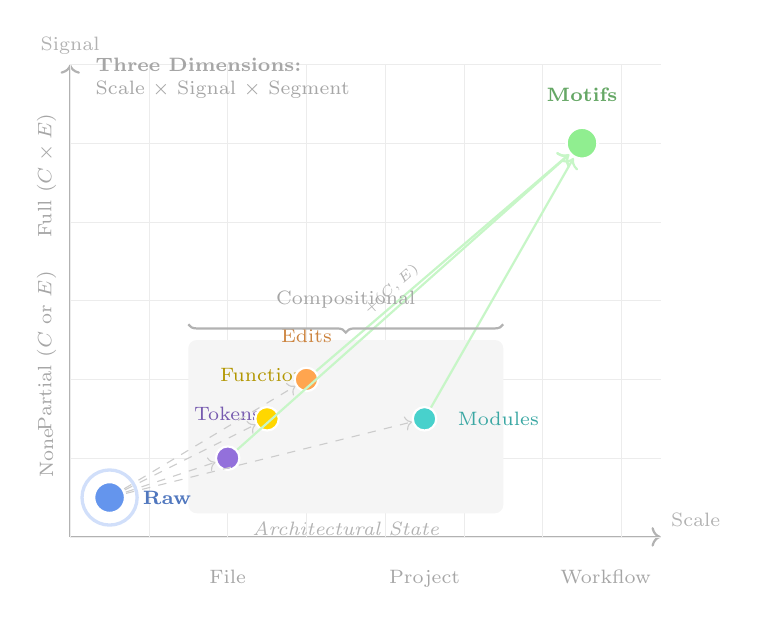
\begin{tikzpicture}[scale=1.0, every node/.style={font=\small}]

% Axes
\draw[->, thick, gray!60] (0,0) -- (7.5,0) node[above right, font=\scriptsize] {Scale};
\draw[->, thick, gray!60] (0,0) -- (0,6) node[above, font=\scriptsize] {Signal};

% Grid (subtle)
\draw[gray!15, very thin] (0,0) grid[step=1] (7.5,6);

% Axis labels
\node[font=\scriptsize, gray!70, anchor=north] at (2,-0.3) {File};
\node[font=\scriptsize, gray!70, anchor=north] at (4.5,-0.3) {Project};
\node[font=\scriptsize, gray!70, anchor=north] at (6.8,-0.3) {Workflow};

\node[font=\scriptsize, gray!70, anchor=east, rotate=90] at (-0.3,1.5) {None};
\node[font=\scriptsize, gray!70, anchor=east, rotate=90] at (-0.3,3.5) {Partial ($C$ or $E$)};
\node[font=\scriptsize, gray!70, anchor=east, rotate=90] at (-0.3,5.5) {Full ($C \times E$)};

% Architectural State region (shaded box)
\fill[gray!8, rounded corners=3pt] (1.5,0.3) rectangle (5.5,2.5);
\node[font=\scriptsize\itshape, gray!60] at (3.5,0.1) {Architectural State};

% Raw (origin - full dimensionality)
\node[circle, fill=rawcolor, inner sep=4pt, draw=white, line width=1pt] (raw) at (0.5,0.5) {};
\node[font=\scriptsize\bfseries, rawcolor!80!black, anchor=west] at (0.8,0.5) {Raw};
\draw[rawcolor!30, very thick] (0.5,0.5) circle (0.35cm);

% File-scale projections (Architectural State)
\node[circle, fill=tokencolor, inner sep=3pt, draw=white, line width=0.8pt] (tokens) at (2,1) {};
\node[font=\scriptsize, tokencolor!80!black, anchor=south] at (2,1.35) {Tokens};

\node[circle, fill=funccolor, inner sep=3pt, draw=white, line width=0.8pt] (funcs) at (2.5,1.5) {};
\node[font=\scriptsize, funccolor!70!black, anchor=south] at (2.5,1.85) {Functions};

\node[circle, fill=editcolor, inner sep=3pt, draw=white, line width=0.8pt] (edits) at (3,2) {};
\node[font=\scriptsize, editcolor!80!black, anchor=south] at (3,2.35) {Edits};

% Project-scale projection (Architectural State)
\node[circle, fill=modcolor, inner sep=3pt, draw=white, line width=0.8pt] (mods) at (4.5,1.5) {};
\node[font=\scriptsize, modcolor!80!black, anchor=west] at (4.8,1.5) {Modules};

% Projection lines from Raw to Architectural State
\draw[->, gray!40, dashed, thin] (raw) -- (tokens);
\draw[->, gray!40, dashed, thin] (raw) -- (funcs);
\draw[->, gray!40, dashed, thin] (raw) -- (edits);
\draw[->, gray!40, dashed, thin] (raw) -- (mods);

% Motifs (enriched with behavioral signals)
\node[circle, fill=motifcolor, inner sep=4pt, draw=white, line width=1pt] (motifs) at (6.5,5) {};
\node[font=\scriptsize\bfseries, motifcolor!70!black, anchor=south] at (6.5,5.4) {Motifs};

% Enrichment arrows (from Architectural State to Motifs)
\draw[->, motifcolor!50, thick] (tokens) -- (motifs) node[midway, sloped, above, font=\tiny, gray!60] {$+ (C, E)$};
\draw[->, motifcolor!50, thick] (edits) -- (motifs);
\draw[->, motifcolor!50, thick] (mods) -- (motifs);
% Legend/annotations
\node[font=\scriptsize, anchor=north west, align=left, gray!70] at (0.2,6.2) {
    \textbf{Three Dimensions:}\\
    Scale $\times$ Signal $\times$ Segment
};

% Scale composition annotation
\draw[decorate, decoration={brace, amplitude=3pt, mirror}, gray!60, thick] 
    (1.5,2.7) -- (5.5,2.7) node[midway, above, font=\scriptsize, gray!70, yshift=2pt] {Compositional};

\end{tikzpicture}

\caption{Representational basis as a vector space.}
\label{fig:vector_space}
\end{figure}

\subsection{Discovering Procedural Patterns with Motifs}

Motifs are recurring patterns that compress complex systems into comparable units. In biology, DNA sequence motifs mark where proteins bind to control genes, compressing thousands of gene interactions into regulatory structures that can be compared across organisms~\cite{alon2007network}. Development motifs work similarly: they compress workflow patterns into reusable sequences, enabling comparison across sessions and composition into larger strategies. Motifs are recurring (appearing across contexts), meaningful (carrying semantic significance beyond surface variation), and composable (combining to form larger structures).

\begin{figure}[!ht]
\centering
\small
\begin{tcolorbox}[colback=white, colframe=gray!50, boxrule=0.5pt, arc=2pt, 
                  left=2pt, right=2pt, top=4pt, bottom=4pt, width=\columnwidth]

\textbf{1. Semantic Projection of Raw Traces}

\vspace{0.3em}
\begin{minipage}{0.48\columnwidth}
    \begin{tcolorbox}[colback=gray!5, colframe=gray!20, boxrule=0.3pt, arc=1pt, left=2pt, right=2pt, top=2pt, bottom=2pt, title={\ttfamily\fontsize{5pt}{5pt}\selectfont Trace A (Refactor)}]
    {\ttfamily\fontsize{5pt}{6pt}\selectfont
    \textcolor{gray}{01} PROMPT "dry utils" \\
    \textcolor{gray}{02} OPEN auth\_utils.ts \\
    \textcolor{gray}{03} EDIT \textcolor{editcolor}{del} validate() \\
    \textcolor{gray}{04} CREATE \textcolor{funccolor}{base.ts} \\
    \textcolor{gray}{05} RUN npm test \textcolor{motifcolor!80!black}{PASS}
    }
    \end{tcolorbox}
\end{minipage}
\hfill
\begin{minipage}{0.48\columnwidth}
    \begin{tcolorbox}[colback=gray!5, colframe=gray!20, boxrule=0.3pt, arc=1pt, left=2pt, right=2pt, top=2pt, bottom=2pt, title={\ttfamily\fontsize{5pt}{5pt}\selectfont Trace B (Feature)}]
    {\ttfamily\fontsize{5pt}{6pt}\selectfont
    \textcolor{gray}{01} PROMPT "move api" \\
    \textcolor{gray}{02} OPEN api\_client.py \\
    \textcolor{gray}{03} OPEN types.py \\
    \textcolor{gray}{04} EDIT \textcolor{editcolor}{del} fetch() \\
    \textcolor{gray}{05} RUN pytest \textcolor{motifcolor!80!black}{PASS}
    }
    \end{tcolorbox}
\end{minipage}

\vspace{0.6em}
\textbf{2. Motif Sequence Alignment (Procedural Diff)}

\vspace{0.2em}
\begin{tcolorbox}[colback=motifcolor!5, colframe=motifcolor!30, boxrule=0.5pt, arc=1pt, left=3pt, right=3pt, top=3pt, bottom=3pt]
\centering
{\ttfamily\fontsize{7pt}{8pt}\selectfont
\begin{tabular}{l@{~~}c@{~~}c@{~~}c@{~~}c@{~~}c}
\textbf{Motif A:} & \colorbox{gray!15}{EXPLORE} & \colorbox{gray!15}{DELETE} & \colorbox{gray!15}{ABSTRACT} & \textemdash & \colorbox{gray!15}{VERIFY} \\
\textbf{Motif B:} & \colorbox{gray!15}{EXPLORE} & \colorbox{gray!15}{DELETE} & \textemdash & \colorbox{red!15}{FIX} & \colorbox{gray!15}{VERIFY} \\
\end{tabular}
}
\end{tcolorbox}

\end{tcolorbox}
\caption{Example of motif ``diffing.''}
\label{fig:motif_alignment}
\end{figure}

\subsubsection{Motif Construction and Properties}

Stability is a property of measurement, and a prerequisite for observability in large-scale systems~\cite{kalman1960observability, forsgren2021space}. In our setting, stability means that the same underlying workflow maps to the same motif under small perturbations such as minor event noise or resampling, so aggregate comparisons remain reliable.

Comparability requires identifying why actions were taken. Real workflows have no predefined labels, so we discover intent from action patterns through clustering. This enables fair comparison: developers solving the same problem may write different code but follow similar strategies, which become visible when workflows are grouped by discovered intent. 

The result is that workflows become searchable by strategy rather than syntax—a developer debugging a type error can find examples from others who tackled similar problems, even across different codebases and languages.  

%This reveals that expertise manifests in procedural patterns, not just in the code artifacts those patterns produce.

We develop a two-stage encoding process for motif discovery.  First, statistical sequence mining extracts recurring structural patterns: PrefixSpan identifies frequent patterns even when separated by unrelated steps, while Sequitur simplifies traces by finding repeated pairs and replacing them with shorthand symbols~\cite{pei2001prefixspan,nevill1997sequitur}. This approach is formalized by the Minimum Description Length principle: recurring patterns can be summarized more compactly, often corresponding to meaningful procedural units~\cite{rissanen1978mdl}. 

Second, intent labels are assigned to clusters after structural abstraction and privacy transformations. Structural patterns make workflows comparable, but they are not inherently meaningful to human readers. Intent labels bridge this gap by attaching semantic meaning to structural patterns, turning opaque sequences into readable strategies. We employ embeddings and hierarchical clustering methods~\cite{campello2015hdbscan, huang2025values}, drawing from the Clio methodology. Event descriptions are embedded in vector space and grouped to surface natural categories. Labels are then assigned by prompting LLMs to summarize the commonalities within each cluster.

This descriptive approach preserves expressiveness and emergent behavior that a fixed taxonomy would suppress. 

%similar to how privacy configurations operate orthogonally.

\section{Characterizing Representations}

Having defined our six encoders and their compositional structure, we now turn to how these representations can be systematically evaluated and compared. Representations make developer workflows legible to both humans and machines. But many representations are possible, and each preserves different information while hiding other details. To reason about which abstraction to use, we introduce measurements that characterize representations along three dimensions: privacy, compression, and utility.

\subsubsection{Privacy} 

In classical privacy settings~\cite{sweeney2002k}, k-anonymity asks how many individuals remain indistinguishable to an observer after data is released. Developer traces are different: they are long sequences of actions whose raw combinations are so specific that nearly every session is unique. At the raw level, the effective entropy is high enough that signal is hard to separate from noise. The objective is not to erase difference, but to suppress irrelevant detail while preserving strategic structure.

Each encoding suppresses detail, widening the set of traces that appear equivalent. Two metrics help characterize this transformation: how much information about a workflow is retained (intra-trace similarity) and how similar that workflow becomes to others after abstraction (inter-trace similarity). Together, these quantities make abstraction levels comparable by revealing how distinctive a trace remains under each encoding.

Reconstruction is typically framed as asking whether a representation preserves enough information to recover a specified target~\cite{bengio2013representation}, mirroring the information bottleneck principle. In the simplest setting, this target is the original trace itself. Under this view, intra-trace similarity plays the role of a reconstruction measure: it quantifies how faithfully the encoded form retains properties of its source.

Inter-trace similarity captures a different but complementary notion. Rather than comparing a trace to its origin, it compares representations across traces of the same type. One can think of this analogously to edit distance metrics such as Levenshtein distance: depending on the abstraction, two workflows may require more or fewer transformations to be considered equivalent. As representations become coarser, distances between traces are expected to shrink because the dimensions along which they can differ are reduced.

\subsubsection{Compression}

Compression measures how much smaller a representation is than the original raw trace, typically in bytes. The compression ratio compares the size of the raw data to the size of its encoding. Reduction occurs in two ways: fewer bytes are stored, and fewer distinct symbols are needed to describe the workflow. Higher compression does not necessarily mean losing useful information. An abstraction can remove syntactic detail while preserving procedural structure. This follows the Minimum Description Length principle: where the quality of a representation is assessed by how well it explains the data while minimizing the total number of bits required to encode both the representation and the data it leaves unexplained. MDL is central to communicating procedural abstractions~\cite{mccarthy2021learning}, where the best-fitting model is the one that can be shared or transferred most efficiently.

\subsubsection{Utility} 

Utility refers to performance on downstream tasks: classification (discovering edit intent, as in code review and PR labeling), retrieval (finding relevant files without accessing raw content, as in agent context selection), and prediction (modeling whether a strategy is likely to succeed).

Because tasks differ, no representation is uniformly best. A format that supports architectural reasoning may be poor for debugging. One that protects privacy may not support reconstruction. Expressiveness describes how much task-relevant information is present in the encoding. Utility depends on whether that information matches the needs of a particular use. An abstraction can remove detail yet become more useful if it exposes the structure required for the task.

Table~\ref{tab:rung_hierarchy} shows that no encoder is universally best; each preserves different information for different purposes. File-scale encoders support questions about specific code, while workflow-scale encoders support questions about strategy. Motifs enable comparison by treating implementation differences as noise, allowing sessions that follow patterns such as “explore → refactor → verify” to be recognized as strategically similar.

This representation framework mirrors abstract interpretation~\cite{cousot1977abstract}, where each encoder defines an abstract domain trading precision for preserved structural patterns. Intent labels bridge the gap between structural patterns and human-understandable meaning by attaching semantic content to opaque sequences, turning them into readable strategies.

\section{Limitations and Discussion}
\label{sec:discussion}

While we focus on Cursor (AI IDE) workflows; extending to terminal agents and CLI tools is one extension. Deploying the companion system to capture and learn from traces would make it possible to see whether recommendation engines built on real-world preferences are valuable. An experiment would be to see whether the wisdom-of-crowds hypotheses holds. 

The core vision is to enable collective learning from developer workflows. Procedural Clio would capture the diversity of programming strategies across many developers. This information could then be used to steer agents specified procedurally from the outset or to power recommendation engines tailored to individual workspaces.

Open questions remain at multiple levels. At the representation level: what is the minimum encoding preserving a given class of patterns? At the learning level: do motifs transfer across languages, teams, or domains? At the systems level: can we detect when developers shift between exploration, implementation, and debugging, adapting encoding accordingly? At the evaluation level, what constitutes a good workflow when developers pursue diverse goals? This work is motivated by the promise of pluralistic systems—those that represent and serve the needs of the collective—where the preferences of different developers can be incorporated into AI systems~\cite{sorensen2024roadmappluralisticalignment}.

\section{Conclusion}

In this work, we study Cursor as an AI-assisted development environment and propose a framework for representing workflows from capture to aggregation. As AI-assisted development becomes ubiquitous, learning from real workflows—not just static artifacts—will shape how systems are built and evaluated. In this regime, context engineering becomes paramount: both humans and agents depend on what context they have access to and how it is represented. Workflow representations provide infrastructure for alignment by making behavior observable while preserving developer control over what to share and how.

\bibliographystyle{ACM-Reference-Format}
\bibliography{references}

\appendix

\section{Representation examples}
\label{sec:representation_examples}

The following progression shows how a single refactoring session transforms from raw telemetry (2,450 bytes) through file-scale and project-scale encoders to procedural motifs (48 bytes), demonstrating the privacy-expressiveness tradeoff. Compression ratios and data sizes are derived from the first author's local companion traces (40,000+ sessions collected over 78 days).

\vspace{0.5em}

\begin{tcolorbox}[colbacktitle={rawcolor!30}, coltitle=black, 
                  colback={rawcolor!5}, colframe={rawcolor}, boxrule=0.5pt,
                  breakable, arc=2pt,
                  title=\textbf{Ground Truth: Raw Events} \hfill {\small 2{,}450 bytes~~$\cdot$~~1$\times$}]
{\ttfamily\scriptsize%
Event: file\_change\\
File: src/utils.ts\\
Timestamp: 2024-01-15T10:23:45Z\\
Diff: +15 lines, -8 lines\\[0.3em]
~~- export function processData(input: string): void \{\\
~~-~~~const result = input.toLowerCase();\\
~~-~~~console.log(result);\\
~~- \}\\[0.2em]
~~+ export async function processData(input: string, options: Config): Promise<string> \{\\
~~+~~~const result = await BaseUtil.process(input, options);\\
~~+~~~return BaseUtil.validate(result);\\
~~+ \}\\[0.3em]
Context: [src/utils.ts, src/api.ts, src/config.ts, \ldots~8 more]%
}

\vspace{0.3em}
{\scriptsize\textit{\textbf{Privacy:} None. \textbf{Reveals:} Full code, exact changes, all metadata. \textbf{Use:} Session debugging.}}
\end{tcolorbox}

\vspace{0.8em}

{\large\textbf{File-Scale Encoders}}

\vspace{0.3em}

\begin{tcolorbox}[colback={tokencolor!5}, colframe={tokencolor!60}, boxrule=0.5pt,
                  arc=2pt, left=3pt, right=3pt, top=4pt, bottom=4pt,
                  title={\bfseries Tokens} \hfill {\small 320 bytes~~$\cdot$~~8$\times$}]
{\ttfamily\scriptsize%
FUNCTION\_DECL:processData $\rightarrow$ ASYNC $\rightarrow$ PARAM:input $\rightarrow$\\
PARAM:options $\rightarrow$ RETURN\_TYPE:Promise $\rightarrow$ AWAIT $\rightarrow$\\
CALL:BaseUtil.process $\rightarrow$ RETURN $\rightarrow$ CALL:BaseUtil.validate%
}

\vspace{0.3em}
{\scriptsize\textit{\textbf{Privacy:} Low. \textbf{Reveals:} Syntax sequences. \textbf{Hides:} Actual identifiers (normalized). \textbf{Use:} Code similarity.}}
\end{tcolorbox}

\vspace{0.5em}

\begin{tcolorbox}[colback={funccolor!5}, colframe={funccolor!60}, boxrule=0.5pt,
                  arc=2pt, left=3pt, right=3pt, top=4pt, bottom=4pt,
                  title={\bfseries Functions} \hfill {\small 185 bytes~~$\cdot$~~13$\times$}]
{\ttfamily\scriptsize%
MODIFY~~processData\\
~~~~~~~~params: (input: string) $\rightarrow$ (input: string, options: Config)\\
~~~~~~~~return: void $\rightarrow$ Promise<string>\\
~~~~~~~~body:~~~[async wrapper added, BaseUtil calls added]\\[0.2em]
ADD~~~~~BaseUtil\\
~~~~~~~~\{process: (input, options) => Promise,~~validate: (result) => string\}\\[0.2em]
DELETE~~deprecatedHelper()%
}

\vspace{0.3em}
{\scriptsize\textit{\textbf{Privacy:} Low. \textbf{Reveals:} Function names, signatures, API changes. \textbf{Hides:} Implementation. \textbf{Use:} API tracking.}}
\end{tcolorbox}

\vspace{0.5em}

\begin{tcolorbox}[colback={editcolor!5}, colframe={editcolor!60}, boxrule=0.5pt,
                  arc=2pt, left=3pt, right=3pt, top=4pt, bottom=4pt,
                  title={\bfseries Edits (Anonymous)} \hfill {\small 95 bytes~~$\cdot$~~26$\times$}]
{\ttfamily\scriptsize%
EDIT(modify) $\rightarrow$ OP:async\_wrapper\\
EDIT(modify) $\rightarrow$ OP:signature\_change\\
EDIT(delete) $\rightarrow$ OP:remove\_function\\
EDIT(create) $\rightarrow$ OP:new\_module%
}

\vspace{0.3em}
{\scriptsize\textit{\textbf{Privacy:} High. \textbf{Reveals:} Operation patterns only. \textbf{Hides:} Function names, files, code. \textbf{Use:} Workflow detection.}}
\end{tcolorbox}

\vspace{0.8em}

{\large\textbf{Project-Scale Encoder}}

\vspace{0.3em}

\begin{tcolorbox}[colback={modcolor!5}, colframe={modcolor!60}, boxrule=0.5pt,
                  arc=2pt, left=3pt, right=3pt, top=4pt, bottom=4pt,
                  title={\bfseries Modules} \hfill {\small 120 bytes~~$\cdot$~~20$\times$}]
{\ttfamily\scriptsize%
Nodes:~~[utils.ts,~~api.ts,~~config.ts,~~models.ts]\\[0.2em]
Edges:~~utils.ts $\rightarrow$ api.ts~~~~~(imports,~~~~~~~~co-edited 5$\times$)\\
~~~~~~~~api.ts $\rightarrow$ config.ts~~~(depends\_on,~~~~co-edited 3$\times$)\\
~~~~~~~~utils.ts $\rightarrow$ models.ts~~(new\_dependency, co-edited 2$\times$)%
}

\vspace{0.3em}
{\scriptsize\textit{\textbf{Privacy:} Medium. \textbf{Reveals:} File relationships, coupling. \textbf{Hides:} Code, function changes. \textbf{Use:} Architecture analysis.}}
\end{tcolorbox}

\vspace{0.8em}

{\large\textbf{Workflow-Scale Encoder}}

\vspace{0.3em}

\begin{tcolorbox}[colbacktitle={motifcolor!30}, coltitle=black,
                  colback={motifcolor!5}, colframe={motifcolor}, boxrule=0.5pt,
                  breakable, arc=2pt,
                  title=\textbf{Motifs (Procedural Strategy)} \hfill {\small 48 bytes~~$\cdot$~~51$\times$}]
{\ttfamily\scriptsize%
PROMPT $\rightarrow$ EXPLORE $\rightarrow$ REFACTOR $\rightarrow$ ABSTRACT $\rightarrow$ TEST $\rightarrow$ COMMIT%
}

\vspace{0.3em}
{\scriptsize%
Intent: \textit{``extract-and-consolidate refactoring''}~~\textcolor{gray}{\textbar}~~Frequency: 23 sessions%
}

\vspace{0.3em}
{\scriptsize\textbf{Behavioral Enrichments:}}
\begin{itemize}[leftmargin=*, itemsep=0pt]
\item {\scriptsize \textbf{Communication ($C$):} \textit{``extract shared validation logic''}}
\item {\scriptsize \textbf{Execution ($E$):} \texttt{npm test} $\rightarrow$ \textcolor{red!60}{FAIL} $\rightarrow$ \textcolor{green!60!black}{PASS}}
\end{itemize}

\vspace{0.3em}
{\scriptsize\textit{\textbf{Privacy:} Highest. \textbf{Reveals:} Workflow strategy only. \textbf{Hides:} All code, files, identifiers. \textbf{Use:} Strategy comparison.}}
\end{tcolorbox}

\vspace{0.5em}

{\scriptsize\textbf{Compression–privacy tradeoff:} As compression increases (1× → 51×), privacy increases (none → highest) while expressiveness shifts from implementation details to procedural patterns.}

\section{Encoder Features}
\begin{table*}[!t]
\centering
\caption{Representation encoders organized by scale and ordered by increasing compression. Compression drives the privacy-expressiveness tradeoff.}
\label{tab:rung_hierarchy}
\small
\renewcommand{\arraystretch}{1.2}
\rowcolors{2}{gray!10}{white}
\begin{tabularx}{\textwidth}{>{\bfseries}l >{\centering\arraybackslash}p{1.2cm} >{\raggedright\arraybackslash}X >{\raggedright\arraybackslash}X >{\raggedright\arraybackslash}X >{\raggedright\arraybackslash}X}
\toprule
\rowcolor{gray!25}
\textbf{Encoder} & \textbf{Scale} & \textbf{What It Tracks} & \textbf{Privacy Level} & \textbf{Primary Use} & \textbf{Extraction Method} \\
\midrule
\rowcolor{rawcolor!15}
Raw & Ground Truth & Complete event logs with all details & None (full data) & Session debugging & Event parsing only \\
\midrule
\multicolumn{6}{c}{\textcolor{gray!60}{\textit{--- File-Scale Encoders (Architectural State) ---}}} \\
\hdashline[0.8pt/2pt]
\rowcolor{tokencolor!15}
Tokens & \textbf{File} & Syntax element sequences & Low (identifiers canonicalized) & Code similarity & Tokenization \\
\rowcolor{funccolor!15}
Functions & \textbf{File} & Specific function changes \textit{with} names and signatures & Low (exposes APIs) & API evolution tracking & Function extraction \\
\rowcolor{editcolor!15}
Edits & \textbf{File} & Operation patterns \textit{without} function names & \textbf{High} (anonymous operations) & Workflow pattern detection & AST parsing \\
\hdashline[0.8pt/2pt]
\midrule
\multicolumn{6}{c}{\textcolor{gray!60}{\textit{--- Project-Scale Encoders (Architectural State) ---}}} \\
\hdashline[0.8pt/2pt]
\rowcolor{modcolor!15}
Modules & \textbf{Project} & File relationships, coupling, co-editing patterns & Medium (structure only) & Dependency analysis & Dependency analysis \\
\hdashline[0.8pt/2pt]
\midrule
\multicolumn{6}{c}{\textcolor{gray!60}{\textit{--- Workflow-Scale Encoders (Procedural Patterns) ---}}} \\
\hdashline[0.8pt/2pt]
\rowcolor{motifcolor!15}
Motifs & \textbf{Workflow} & Procedural strategies enriched with prompts ($C$) and execution ($E$) & \textbf{Highest} (patterns only) & Strategy comparison & Sequence mining + clustering \\
\hdashline[0.8pt/2pt]
\bottomrule
\end{tabularx}
\vspace{0.3em}
{\scriptsize \textit{Encoders within the dotted box compose into the ``structural'' dimension in the space of representations. All representations can be enriched with additional privacy and semantic transformations.}}
\end{table*}

\end{document}
